\documentclass[12pt, titlepage]{article}

\usepackage{booktabs}
\usepackage{tabularx}
\usepackage{hyperref}
\usepackage{amsfonts}
\usepackage{amssymb}
\usepackage{graphicx}
\usepackage{float}
\usepackage{colortbl}
\usepackage{xr}
\hypersetup{
    colorlinks,
    citecolor=blue,
    filecolor=black,
    linkcolor=red,
    urlcolor=blue
}
\usepackage[round]{natbib}
\usepackage{graphicx}
\usepackage{caption}


%% Comments

\usepackage{color}

\newif\ifcomments\commentstrue %displays comments
%\newif\ifcomments\commentsfalse %so that comments do not display

\ifcomments
\newcommand{\authornote}[3]{\textcolor{#1}{[#3 ---#2]}}
\newcommand{\todo}[1]{\textcolor{red}{[TODO: #1]}}
\else
\newcommand{\authornote}[3]{}
\newcommand{\todo}[1]{}
\fi

\newcommand{\wss}[1]{\authornote{blue}{SS}{#1}} 
\newcommand{\plt}[1]{\authornote{magenta}{TPLT}{#1}} %For explanation of the template
\newcommand{\an}[1]{\authornote{cyan}{Author}{#1}}

%% Common Parts

\newcommand{\progname}{2D Localizer} % PUT YOUR PROGRAM NAME HERE
\newcommand{\authname}{Aliyah Jimoh} % AUTHOR NAMES                  

\usepackage{hyperref}
    \hypersetup{colorlinks=true, linkcolor=blue, citecolor=blue, filecolor=blue,
                urlcolor=blue, unicode=false}
    \urlstyle{same}
                                


\begin{document}

\title{System Verification and Validation Plan for \progname} 
\author{Aliyah Jimoh}
\date{\today}
	
\maketitle

\pagenumbering{roman}

\section*{Revision History}

\begin{tabularx}{\textwidth}{p{3cm}p{2cm}X}
\toprule {\bf Date} & {\bf Version} & {\bf Notes}\\
\midrule
24/02/2025 & 1.0 & Initial Draft\\
03/03/2025 & 1.1 & Feedback Implementation\\
\bottomrule
\end{tabularx}

~\\

\newpage

\tableofcontents

\listoftables

\listoffigures
\wss{Remove this section if it isn't needed}

\newpage

\section{Symbols, Abbreviations, and Acronyms}

\renewcommand{\arraystretch}{1.2}
\begin{tabular}{l l} 
  \toprule		
  \textbf{Symbol} & \textbf{Description}\\
  \midrule 
  2D & Two-Dimensional \\
  \progname & 2D Localization Solution\\
  CRLB & Cram\'er-Rao Lower Bound\\
  FM & Fiducial Marker \\
  GTSAM & Georgia Tech Smoothing and Mapping\\
  MG & Module Guide \\
  MIS & Module Interface Specification \\
  MLE & Maximum Likelihood Estimation\\
  PEP8 & Python Enhancement Proposal 8 \\
  RMSE & Root Mean Squared Error\\
  SRS & Software Requirements Specification\\
  T & Test\\
  VnV & Verification and Validation\\
  $N$ & Number of beacons used \\
  $\mathbf{\hat{x}}$ & estimated robot pose ($x, y, \theta$)\\
  $\tilde{\mathbf{d}}$ & $\mathbb{R}^N$ vector of a set of range measurements\\
  $\mathbf{T}_{wf}$ & pose of fiducial marker in worlds frame \\
  $\mathbf{T}_{fr}$ & pose of fiducial marker in robot frame  \\
  $\mathbf{T}_{wr}$ & pose of robot in world frame  \\
  \bottomrule
\end{tabular}\\

For a full list of symbols, abbreviations, and acronyms used, refer to section 1 in the \href{https://github.com/AliyahJimoh/2D-Localizer/blob/main/docs/SRS/SRS.pdf}{SRS} document.

\newpage

\pagenumbering{arabic}

This document shows the verification and validation plan of the \progname~program. This plan starts with general information that talks about \progname~in section \ref{sec_general}. The plan and system tests involved with this software is explained in sections \ref{sec_plan} and \ref{sec_sys-tests}.



\section{General Information}\label{sec_general}

\subsection{Summary}

This document examines the verification and validation plan of \progname. This software is used to help accurately locate mobile robots in a provided 2D map given the measurements and coordinates of the sensors and fiducial markers (FMs).

\subsection{Objectives}

The objective of this plan is to validate the accuracy of this program to build confidence in the software's reliability and performance. This plan also aims to satisfy all the requirements from the System Requirements Specification (\href{https://github.com/AliyahJimoh/2D-Localizer/blob/main/docs/SRS/SRS.pdf}{SRS}).  

% \wss{State what is intended to be accomplished.  The objective will be around
%   the qualities that are most important for your project.  You might have
%   something like: ``build confidence in the software correctness,''
%   ``demonstrate adequate usability.'' etc.  You won't list all of the qualities,
%   just those that are most important.}

% \wss{You should also list the objectives that are out of scope.  You don't have 
% the resources to do everything, so what will you be leaving out.  For instance, 
% if you are not going to verify the quality of usability, state this.  It is also 
% worthwhile to justify why the objectives are left out.}

% \wss{The objectives are important because they highlight that you are aware of 
% limitations in your resources for verification and validation.  You can't do everything, 
% so what are you going to prioritize?  As an example, if your system depends on an 
% external library, you can explicitly state that you will assume that external library 
% has already been verified by its implementation team.}

\subsection{Challenge Level and Extras}

This system has an advanced research level which can be seen from the implementation and the topic. Setting up the robot’s movement, accurately displaying the trajectory, and coordinating sensor measurements each introduce their own level of complexity. Additionally, finding a way to animate the output adds further difficulty to the system. However, the topic is not niche meaning that there are papers and libraries available that can be used for guidance and inspiration.

% \wss{State the challenge level (advanced, general, basic) for your project.
% Your challenge level should exactly match what is included in your problem
% statement.  This should be the challenge level agreed on between you and the
% course instructor.  You can use a pull request to update your challenge level
% (in TeamComposition.csv or Repos.csv) if your plan changes as a result of the
% VnV planning exercise.}

% \wss{Summarize the extras (if any) that were tackled by this project.  Extras
% can include usability testing, code walkthroughs, user documentation, formal
% proof, GenderMag personas, Design Thinking, etc.  Extras should have already
% been approved by the course instructor as included in your problem statement.
% You can use a pull request to update your extras (in TeamComposition.csv or
% Repos.csv) if your plan changes as a result of the VnV planning exercise.}

\subsection{Relevant Documentation}

% \wss{Reference relevant documentation.  This will definitely include your SRS
%   and your other project documents (design documents, like MG, MIS, etc).  You
%   can include these even before they are written, since by the time the project
%   is done, they will be written.  You can create BibTeX entries for your
%   documents and within those entries include a hyperlink to the documents.}

% \citet{SRS}

% \wss{Don't just list the other documents.  You should explain why they are relevant and 
% how they relate to your VnV efforts.}

The documentation relevant to the \progname~includes the Problem Statement since it explains the proposed software, the \href{https://github.com/AliyahJimoh/2D-Localizer/blob/main/docs/SRS/SRS.pdf}{SRS} which talks about the requirements needed to properly use the system, the Verification and Validation (\href{https://github.com/AliyahJimoh/2D-Localizer/blob/main/docs/VnVReport/VnVReport.pdf}{VnV}) report that goes through the tests and plans for the system, and the Module Guide (\href{https://github.com/AliyahJimoh/2D-Localizer/blob/main/docs/Design/SoftArchitecture/MG.pdf}{MG}) and Module Interface Specification (\href{https://github.com/AliyahJimoh/2D-Localizer/blob/main/docs/Design/SoftDetailedDes/MIS.pdf}{MIS}) for the design.

\section{Plan}\label{sec_plan}

This section describes the tests made for the \progname~system. This begins by mentioning the VnV team in section~\ref{vnv_team}, then followed by the SRS Verification Plan in~\ref{plan_SRS}, the Design Verification Plan in section~\ref{plan_design},the VnV Plan Verification Plan in section~\ref{plan_verification}, the Implementation Verification Plan in section~\ref{plan_implement}, the Automated Testing and Verification tools in section~\ref{plan_auto}, and the Software Validation Plan in section~\ref{plan_software}.

\subsection{Verification and Validation Team}\label{vnv_team}

This section shows the members of the VnV team. They are shown in Table \ref{table:vnvTeam} along with what document they contributed in and their roles.

\begin{center}
  \begin{table}[h]
    \centering
    
    \begin{tabular}{|l|l|p{5cm}|}
        \hline
        \textbf{Name} & \textbf{Document} & \textbf{Role} \\
        \hline
        Aliyah Jimoh & All & Author\\
        \hline
        Dr.~Spencer Smith & All & Instructor \\
                          &     & Reviewer\\
        \hline
        Kiran Singh & SRS & Domain Expert\\
                    & VnV & Reviewer      \\
                    & MG &       \\
                    & MIS &       \\
        \hline
        Dr.~Matthew Giamou & Problem Statement & Supervisor \\
                           &                   & Reviewer \\
        \hline
    \end{tabular}

    \caption{Verification and Validation Team}
    \label{table:vnvTeam}
\end{table}
\end{center}

\subsection{SRS Verification Plan}\label{plan_SRS}

The SRS document for \progname~will be verified through the following steps:
\begin{enumerate}
  \item The initial review will be performed by the assigned reviewers (Dr.~Spencer Smith and Kiran Singh) and will use the \href{https://github.com/AliyahJimoh/2D-Localizer/blob/main/docs/Checklists/SRS-Checklist.pdf}{SRS Checklist} as a guide.
  \item The reviewers will give feedback through creating issues in the GitHub repository.
  \item The author (Aliyah Jimoh) will apply the feedback to the document and address issues that may not be applied.
  \item The author will discuss with the supervisor (Dr.~Matthew Giamou) and ask for their input.
\end{enumerate}

% \wss{If you have a supervisor for the project, you shouldn't just say they will
% read over the SRS.  You should explain your structured approach to the review.
% Will you have a meeting?  What will you present?  What questions will you ask?
% Will you give them instructions for a task-based inspection?  Will you use your
% issue tracker?}

% \wss{Maybe create an SRS checklist?}

\subsection{Design Verification Plan}\label{plan_design}
The design for \progname~will be verified through the following steps:
\begin{enumerate}
  \item The design documents, the MG and MIS, will be reviewed by the assigned reviewers (Kiran Singh and Dr.~Spencer Smith) and will use both checklists (\href{https://github.com/AliyahJimoh/2D-Localizer/blob/main/docs/Checklists/MG-Checklist.pdf}{MG Checklist} and \href{https://github.com/AliyahJimoh/2D-Localizer/blob/main/docs/Checklists/MIS-Checklist.pdf}{MIS Checklist}) as a guide.
  \item The reviewers will give feedback through creating issues in the GitHub repository.
  \item The author (Aliyah Jimoh) will apply the feedback to the document and address issues that may not be applied.
\end{enumerate}

% \wss{Plans for design verification}

% \wss{The review will include reviews by your classmates}

% \wss{Create a checklist?}

\subsection{Verification and Validation Plan Verification Plan}\label{plan_verification}

The VnV plan for \progname~will be verified through the following steps:
\begin{enumerate}
  \item The VnV plan will be reviewed by the assigned reviewers (Kiran Singh and Dr.~Spencer Smith) and will use the \href{https://github.com/AliyahJimoh/2D-Localizer/blob/main/docs/Checklists/VnV-Checklist.pdf}{VnV Checklist} as a guide.
  \item The reviewers will give feedback through creating issues in the GitHub repository.
  \item The author (Aliyah Jimoh) will apply the feedback to the document and address issues that may not be applied.
\end{enumerate}

% \wss{The verification and validation plan is an artifact that should also be
% verified.  Techniques for this include review and mutation testing.}

% \wss{The review will include reviews by your classmates}

% \wss{Create a checklists?}

\subsection{Implementation Verification Plan}\label{plan_implement}

The implementation of \progname~will be verified be the following techniques:
\begin{itemize}
  \item \textbf{Static Verification}
  \newline  
    The author will perform a user demonstration to the domain expert (Kiran Singh) and go through different tests to check the accuracy. The author will then do a user test case in a presentation while explaining the tests made and performed. Section \ref{sec_sys-tests} describes system-level tests derived from SRS functional requirements that are implemented through code in Section \ref{unit-test} and validated through dynamic testing.

  \item \textbf{Dynamic Testing}
  \newline
  The unit tests for \progname~are discussed in section \ref{unit-test} 

\end{itemize}

% \wss{You should at least point to the tests listed in this document and the unit
%   testing plan.}

% \wss{In this section you would also give any details of any plans for static
%   verification of the implementation.  Potential techniques include code
%   walkthroughs, code inspection, static analyzers, etc.}

% \wss{The final class presentation in CAS 741 could be used as a code
% walkthrough.  There is also a possibility of using the final presentation (in
% CAS741) for a partial usability survey.}

\subsection{Automated Testing and Verification Tools}\label{plan_auto}

\subsubsection{Code Guidelines}
For Python implementation, the 2D Localization software will follow the coding style guidelines outlined in Python Enhancement Proposal 8 (PEP8). To enforce this, the Flake8 linter will be used to ensure that code meets PEP8's guidelines and for continuous integration in GitHub Actions.

\subsubsection{GTSAM Integration}
Georgia Tech Smoothing and Mapping (\href{https://github.com/borglab/gtsam}{GTSAM}) by~\cite{gtsam2022} is a library that implements sensor fusion for robotics using factor graphs. These graphs consist of two types of nodes: variables (e.g., robot poses and sensor measurements) and factors, which represent probabilistic constraints between them. \progname~will be using this library as a modelling language and would need to run unit tests to verify if GTSAM is properly integrated.

\begin{figure}[H]
  \begin{center}
    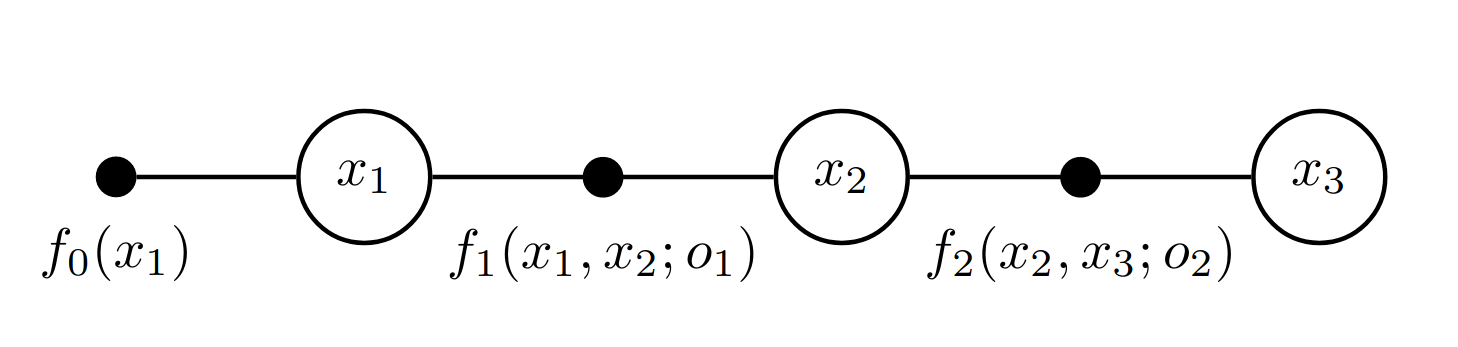
\includegraphics[width=0.6\textwidth]{factor_graph.png}
    \caption{Example Factor Graph from \cite{Dellaert2012}}
    \label{fig_factor} 
  \end{center}
\end{figure}

\subsubsection{Automated Testing}
Unit testing for \progname~is implemented using the \texttt{pytest} framework. This tool enables automatic test discovery, detailed failure reporting, and integration with coverage tools. These tests verify functional and non-functional requirements dynamically and are executed regularly through continuous integration.


% \wss{What tools are you using for automated testing.  Likely a unit testing
%   framework and maybe a profiling tool, like ValGrind.  Other possible tools
%   include a static analyzer, make, continuous integration tools, test coverage
%   tools, etc.  Explain your plans for summarizing code coverage metrics.
%   Linters are another important class of tools.  For the programming language
%   you select, you should look at the available linters.  There may also be tools
%   that verify that coding standards have been respected, like flake9 for
%   Python.}

% \wss{If you have already done this in the development plan, you can point to
% that document.}

% \wss{The details of this section will likely evolve as you get closer to the
%   implementation.}

\subsection{Software Validation Plan}\label{plan_software}

To help validate the accuracy of the localization algorithm, \progname~will use predefined 2D trajectory data in CSV format. These files contain ground truth positions that are used to compare against estimated poses generated by the system. If suitable datasets are not available, alternate test cases and validation procedures will be discussed with the supervisor.

\section{System Tests}\label{sec_sys-tests}

This section goes over the different system tests \progname~will go through to satisfy its requirements.

\subsection{Tests for Functional Requirements}

This subsection looks at the system tests that will help satisfy the functional requirements outlined in the SRS (Section 5.1)

\subsubsection{Sensor Estimation Tests}

% \wss{It would be nice to have a blurb here to explain why the subsections below
%   cover the requirements.  References to the SRS would be good here.  If a section
%   covers tests for input constraints, you should reference the data constraints
%   table in the SRS.}

  % These tests cover the requirements R1 to R3
		
\paragraph{Range-Only Pose Estimation}

\begin{enumerate}

\item{\textbf{F-RO-01}}

\textbf{Requirements Addressed:} R3, R5\\
\textbf{Control:} Automatic
					
\textbf{Initial State: }
\begin{itemize}
  \item Known beacon positions
  \item Robot starts at unknown location
\end{itemize}
					
\textbf{Input:} A set of noisy range measurements $\mathbf{\tilde{d}_j}$ with each set containing the number of beacons that whose range detected it. The map size is given along with the initial estimate position of the robot. All inputs are derived from a predefined YAML configuration file.

\textbf{Output:} The estimated robot pose $\mathbf{\hat{x}}$ represented by $(x,y,\theta)$, corresponding to the robot's position and heading in the environment.
 

\textbf{Test Case Derivation:} SRS Section IM2
					
\textbf{How test will be performed:} The tester will run the program with a valid input YAML file containing beacon positions, trajectory data, and noise configuration. The system will estimate a pose using only range measurements. The test is considered a pass if:
\begin{itemize}
  \item A valid pose estimate is returned (finite values)
  \item The pose lies within the bounds of the map dimensions
\end{itemize}

\end{enumerate}


\paragraph{SE(2) Transformation Estimation}
\begin{enumerate}					
\item{F-SE2-01}

\textbf{Requirements Addressed:} R2, R5\\
\textbf{Control:} Automatic
					
Initial State: 
\begin{itemize}
  \item Robot starts with a known pose $T_{wr}$
  \item Fiducial markers are placed at fixed positions $T_{wf}$
\end{itemize}
					
Input: Transformation matrices $T_{wf}, T_{fr}$ 

Output: Computed transformation must satisfy:
\[
T_{wr} = T_{wf} T_{fr}
\]

Test Case Derivation: SRS Section IM3

How test will be performed: The tester will configure an input YAML file where the robot has line-of-sight to fiducial markers (FMs). The system will use this to refine its pose estimate. The test passes if:
\begin{itemize}
  \item A pose is returned without error
  \item Estimated heading shows consistent improvement compared to range-only results
  \item The result remains finite and within bounds
\end{itemize}
\end{enumerate}

\paragraph{Range + SE(2) Sensor Fusion Test}
\begin{enumerate}
\item{F-SF-01}

\textbf{Requirements Addressed:} R5, R6\\
\textbf{Control:} Automatic
					
Initial State: 
\begin{itemize}
  \item Robot starts at unknown pose
  \item Beacons and fiducial markers placed in test environment
\end{itemize}
					
Input: Range measurements + SE(2) transformation constraints

Output: Estimated pose $T_{wr}$ and $\hat{x}$. RMSE and CRLB metrics are used to assess accuracy improvement over range-only estimation.

Test Case Derivation: F-RO-01 and F-SE2-01

How test will be performed: The tester will provide input files with both fiducial and range data, and compare the results against a previous run using only range data. The factor graph includes range-based constraints (on distance to beacons) and FM based constraints, represented as BetweenFactors on pose nodes. The test passes if:
\begin{itemize}
  \item The fused system produces a pose estimate without failure
  \item The test compares differences in estimated pose between range-only and fused approaches, quantified by RMSE and CRLB.
  \item Accuracy improves or remains consistent as measured by the CRLB matrix.
\end{itemize}

\end{enumerate}

\subsubsection{Input Testing}
\paragraph{Input Validation}

\begin{enumerate}

\item{\textbf{F-IN-01}}

\textbf{Requirements Addressed:} R4\\
\textbf{Control:} Automatic
					
\textbf{Initial State: }
\begin{itemize}
  \item Uninitialized or corrupted input files.
\end{itemize}
					
\textbf{Input:} Malformed YAML or invalid numeric data in CSV files.

\textbf{Output:} System-generated error message or exception
					
\textbf{How test will be performed:} The tester will intentionally modify the input YAML and/or CSV files to introduce syntax errors, negative or NaN values, or structurally invalid fields. The system should raise an error and refuse to proceed. The test passes if:
\begin{itemize}
  \item An informative error is shown
  \item The system halts without crashing or proceeding with incorrect data
\end{itemize}

\end{enumerate}

\subsubsection{Visual Testing}
% This test covers the requirement R5

\paragraph{2D Map Overlay of Estimated Poses}
\begin{enumerate}					
\item{F-MO-01}

\textbf{Requirements Addressed:} R1, R2, R7, R9\\
\textbf{Control:} Automatic
					
\textbf{Initial State: }
\begin{itemize}
  \item Environment 2D map and sensor locations (beacons, fiducials) are known.
  \item Robot follows a predefined trajectory.
\end{itemize}
					
Input: \begin{itemize}
  \item Ground truth trajectory $T_{wr}$
  \item Estimated trajectory from localization output $\hat{x}$, generated by a GTSAM-based factor graph optimization.
  \item Sensor positions and detections.
\end{itemize}

Output: The visualization correctly displays:
\begin{itemize}
    \item Estimated trajectory $\hat{x}$ based on GTSAM’s factor graph optimization.
    \item Sensor placements (beacons, fiducial markers).
\end{itemize}

Test Case Derivation: The estimated pose $\hat{x}$ is computed using Maximum Likelihood Estimation (MLE), as described in SRS Section IM2.

\textbf{How test will be performed:} The tester will launch the visualization after localization completes. The test passes if:
\begin{itemize}
  \item The map is displayed without error
  \item All landmarks are plotted correctly
  \item The trajectory follows the expected path smoothly
  \item The robot's position updates dynamically.
\end{itemize}

\end{enumerate}

\paragraph{Real-Time Pose Display}

\begin{enumerate}

\item{\textbf{F-RT-01}}

\textbf{Requirements Addressed:} R8\\
\textbf{Control:} Manual
					
\textbf{Initial State: }Live localization process is running 
					
\textbf{Input:} Pose estimates that are generated over time

\textbf{Output:} Updated GUI table showing ($x, y, \theta$) at each position.
					
\textbf{How test will be performed:} The tester will observe the GUI during runtime. The test passes if:
\begin{itemize}
  \item The table updates with each new pose
  \item Updates occur at consistent intervals
  \item No freezes or lag are observed
\end{itemize}

\end{enumerate}

\subsection{Tests for Nonfunctional Requirements}

\subsubsection{Estimation Accuracy}
		
\paragraph{Accuracy Validation}

\begin{enumerate}

\item{\textbf{NF-ACC-01}}

\textbf{Requirements Addressed:} R6, NFR1\\
\textbf{Type:} Nonfunctional, Dynamic, Automatic
					
Initial State: Final pose estimate has been computed.
					
Input/Condition: 
\begin{itemize}
  \item Sensor data (real or simulated).
  \item Estimated robot poses $\hat{x}$, generated using a GTSAM-based factor graph optimization.
  \item Ground truth trajectory.
\end{itemize}
					
Output/Result: 
\begin{itemize}
  \item The Root Mean Squared Error (RMSE) of the estimated poses $\hat{x}$ must satisfy the accuracy constraint in SRS Section 5.2, Requirement NFR1.
  \item The estimated pose covariance must not exceed the theoretical Cram\'er-Rao Lower Bound (CRLB) (SRS Section TM2).
\end{itemize}
					
\textbf{How test will be performed:} The tester will run the system with a test configuration containing known ground truth data and noise-defined sensor measurements. The system will estimate poses using factor graph optimization.
\begin{itemize}
  \item RMSE satisfies the required accuracy threshold
  \item The CRLB matrix is finite and does not exceed the expected theoretical bound.
\end{itemize}

\end{enumerate}

\subsubsection{Maintainability}
\begin{enumerate}
  \item \textbf{NF-MAINT-01}  \\
  \textbf{Requirements Addressed:} NFR2 \\
  \textbf{Control:} Manual
  
  \textbf{Initial State:} A tested and working version of the system is available.
  
  \textbf{Input:} A change is made to a single module (e.g., M2 - GTSAM) such as modifying the function or sensor input structure.
  
  \textbf{Output:} The system continues to operate correctly and all previously passing unit tests remain successful.
  
  \textbf{How test will be performed:}  
  The tester will intentionally modify a component (e.g., replace a function in \texttt{gtsam\_wrapper.py}) and rerun the unit tests using \texttt{pytest}. The system passes if:  
  \begin{itemize}
      \item The modified component functions as intended 
      \item No regressions occur in unrelated modules (e.g., test failures in M3, M8, M9).
  \end{itemize}
\end{enumerate}

\subsubsection{Usability}
\begin{enumerate}
  \item \textbf{NF-USE-01}  \\
  \textbf{Requirements Addressed:} NFR3 \\
  \textbf{Control:} Manual

  \textbf{Initial State:} A user with access to a clean Linux or macOS environment and Git is ready to install the system.

  \textbf{Input:} The user clones the repository and runs the Makefile with the command \texttt{make install test}.

  \textbf{Output:} The software environment is successfully set up and all unit tests pass.

  \textbf{How test will be performed:}  
  On both Linux and macOS machines, the tester will:  
  \begin{enumerate}
      \item Clone the repository from GitHub.  
      \item Run \texttt{make install} to initialize the environment and install dependencies.  
      \item Run \texttt{make test} to confirm functionality.  
  \end{enumerate}
  The test passes if all steps complete without error and the output logs show successful test execution.
\end{enumerate}

\newpage
\subsection{Traceability Between Test Cases and Requirements}

\begin{table}[h!]
  \centering
  \resizebox{\textwidth}{!}{
    \begin{tabular}{|c|c|c|c|c|c|c|c|c|c|}
      \hline
        & F-RO-01 & F-SE2-01 & F-SF-01 & F-IN-01 & F-MO-01 & F-RT-01 &NF-ACC-01 & NF-MAINT-01 & NF-USE-01\\
      \hline
      R1      & & & &X &X & & & & \\ \hline
      R2      & &X & &X & & & & & \\ \hline
      R3      &X & & &X & & & & & \\ \hline
      R4      & & & &X & & & & & \\ \hline
      R5      &X &X &X & & & & & & \\ \hline
      R6      & & &X & & & &X & & \\ \hline
      R7      & & & & &X & & & & \\ \hline
      R8      & & & & &X &X & & & \\ \hline
      R9      & & & & &X & & & & \\ \hline
      NFR1      & & & & & & &X & & \\ \hline
      NFR2      & & & & & & & &X & \\ \hline
      NFR3      & & & & & & & & & X\\ 
      \hline
      \end{tabular}
  }
  \caption{Traceability Matrix Showing the Connections Between Requirements and System Tests}
\end{table}


\section{Unit Test Description}\label{unit-test}

% \wss{This section should not be filled in until after the MIS (detailed design
%   document) has been completed.}

% \wss{Reference your MIS (detailed design document) and explain your overall
% philosophy for test case selection.}  

% \wss{To save space and time, it may be an option to provide less detail in this section.  
% For the unit tests you can potentially layout your testing strategy here.  That is, you 
% can explain how tests will be selected for each module.  For instance, your test building 
% approach could be test cases for each access program, including one test for normal behaviour 
% and as many tests as needed for edge cases.  Rather than create the details of the input 
% and output here, you could point to the unit testing code.  For this to work, you code 
% needs to be well-documented, with meaningful names for all of the tests.}

This section describes how the unit tests verify software components in \progname~as described in the MIS. Unit testing is conducted dynamically using the pytest framework and is focused on verifying that each function behaves correctly under normal and invalid conditions. Each test corresponds to one or more functional or nonfunctional requirements described in the SRS.

All test cases can be found in the \href{https://github.com/AliyahJimoh/2D-Localizer/tree/main/test}{test} directory of the repository, with descriptive names and in-code docstrings referencing their Test IDs.

\subsection{Unit Testing Scope}

% \wss{What modules are outside of the scope.  If there are modules that are
%   developed by someone else, then you would say here if you aren't planning on
%   verifying them.  There may also be modules that are part of your software, but
%   have a lower priority for verification than others.  If this is the case,
%   explain your rationale for the ranking of module importance.}

The focus of unit testing is on modules M3 (Input Format), M6 (Localization), M8 (Plotting), and M9 (Accuracy Evaluation).

Modules like M2 (GTSAM) and M7 (Control Module) are not explicitly tested at the unit level since they act primarily as libraries or orchestration logic. M4 (Simulation) as its output's behaviour is indirectly validated through localization, accuracy and visualization tests M5 (Output Format) is not unit-tested because it primarily writes to a GUI table which is a side-effect operation better validated through manual inspection or system-level tests.

\subsection{Tests for Functional Requirements}

% \wss{Most of the verification will be through automated unit testing.  If
%   appropriate specific modules can be verified by a non-testing based
%   technique.  That can also be documented in this section.}

\subsubsection{Module 3: Input Format}

% \wss{Include a blurb here to explain why the subsections below cover the module.
%   References to the MIS would be good.  You will want tests from a black box
%   perspective and from a white box perspective.  Explain to the reader how the
%   tests were selected.}
Module 3 handles parsing and validation of user-provided inputs, including YAML files, sensor positions, and measurement arrays. Tests confirm input correctness, formatting, and rejection of invalid files using both black-box and white-box strategies.

\begin{enumerate}

\item{test\_invalid\_yaml (from \texttt{test\_input\_file.py})\\}

Type: Functional, Dynamic, Automatic
					
Initial State: User provides a malformed input file (e.g., YAML with syntax error or NaNs in CSV)
					
Input: Invalid YAML or malformed CSV file
					
Output: Raised exception or error message

Test Case Derivation: From R4 - the system must reject malformed files

How test will be performed: Automatic test using PyTest
					
\item{test\_map\_image (from \texttt{test\_inputs.py})\\}

Type: Functional, Dynamic, Automatic
					
Initial State: User provides a YAML file with a valid map path
					
Input: Valid YAML file referencing a .png or .jpg map
					
Output: File existence confirmed

Test Case Derivation: From R4 - the system must reject malformed files

How test will be performed: Automatic test using PyTest

\item{test\_coordinates (from \texttt{test\_inputs.py})\\}

Type: Functional, Dynamic, Automatic
					
Initial State: YAML and CSV files include sensor coordinates
					
Input: 2D coordinate arrays
					
Output: Parsed as float arrays of shape (N, 2)

Test Case Derivation: From R2

How test will be performed: Automatic test using PyTest

\item{test\_range\_measurements (from \texttt{test\_inputs.py})\\}

Type: Functional, Dynamic, Automatic
					
Initial State: Range matrix and trajectory arrays provided
					
Input: 2D range array ($\mathbf{\tilde{d}_j}$), trajectory
					
Output: Dimensions and type validity confirmed

Test Case Derivation: From R3

How test will be performed: Automatic test using PyTest
    
\end{enumerate}

\subsubsection{Module 6: Localization}

Module 6 implements the pose estimation logic using range and fiducial data. Tests validate localization output under different sensor configurations through both structural and behavioural checks.

\begin{enumerate}
  \item{test\_range\_only (from \texttt{test\_estimated\_position.py})}

  Type: Functional, Dynamic, Automatic
            
  Initial State:  
  \begin{itemize}
    \item Robot pose is unknown.
    \item Only beacon data is used.
  \end{itemize}
            
  Input: Range measurements from beacons
            
  Output: Estimated pose $(x, y, \theta)$
  
  Test Case Derivation: IM2 from SRS
  
  How test will be performed: Automatic test using PyTest
            
  \item{test\_fiducials (from \texttt{test\_estimated\_position.py})}
  
  Type: Functional, Dynamic, Automatic
            
  Initial State: Robot starts near FMs
            
  Input: Relative SE(2) transformations to FMs
            
  Output: Refined pose using FM constraints
  
  Test Case Derivation: IM3 from SRS
  
  How test will be performed: Automatic test using PyTest
  
  \item{test\_sensor\_fusion (from \texttt{test\_estimated\_position.py})}
  
  Type: Functional, Dynamic, Automatic
            
  Initial State: Robot has access to both range and fiducial data
            
  Input: Combined measurements
            
  Output: Pose with both contributions
  
  Test Case Derivation: Merged result of IM2 + IM3 from SRS
  
  How test will be performed: Automatic test using PyTest
\end{enumerate}

\subsubsection{Module 8: Plotting}
Module 8 handles visual output of the localization process. The test checks that visualization completes without crashing and overlays are displayed. The unit test ensures plotting functions render without error and support diagnostic overlays.

\begin{enumerate}
  \item {\texttt{test\_visualization()} (from \texttt{test\_visuals.py})}
  
  Type: Functional, Dynamic, Automatic
            
  Initial State: Estimated pose is computed using GTSAM
            
  Input: Robot pose estimate, beacon layout, noise variances, and ground truth trajectory
            
  Output: RMSE scalar, FIM matrix, and CRLB matrix
  
  Test Case Derivation: From R7 and R9 – visualization must reflect estimated results in real-time and overlay trajectories.
  
  How test will be performed: Automatic test using PyTest
\end{enumerate}



\subsection{Tests for Nonfunctional Requirements}

% \wss{If there is a module that needs to be independently assessed for
%   performance, those test cases can go here.  In some projects, planning for
%   nonfunctional tests of units will not be that relevant.}

% \wss{These tests may involve collecting performance data from previously
%   mentioned functional tests.}

\subsubsection{Module 9: Accuracy Evaluation}
Module 9 evaluates estimation accuracy using FIM and CRLB metrics. Tests check numerical soundness and compliance with statistical requirements.

\begin{enumerate}
  \item {\texttt{test\_accuracy()} (from \texttt{test\_accuracy.py})}
  
  Type: Functional, Dynamic, Automatic
            
  Initial State: Estimated pose is computed using GTSAM
            
  Input: Robot pose estimate, beacon layout, noise variances, and ground truth trajectory
            
  Output: RMSE scalar, FIM matrix, and CRLB matrix
  
  Test Case Derivation: From NFR1 and TM2 in the SRS
  
  How test will be performed: Automatic test using PyTest
\end{enumerate}


% \subsubsection{Module ?}
		
% \begin{enumerate}

% \item{test-id1\\}

% Type: \wss{Functional, Dynamic, Manual, Automatic, Static etc. Most will
%   be automatic}
					
% Initial State: 
					
% Input/Condition: 
					
% Output/Result: 
					
% How test will be performed: 
					
% \item{test-id2\\}

% Type: Functional, Dynamic, Manual, Static etc.
					
% Initial State: 
					
% Input: 
					
% Output: 
					
% How test will be performed: 

% \end{enumerate}

% \subsubsection{Module ?}

% ...

\subsection{Traceability Between Test Cases and Modules}

\begin{table}[h!]
  \centering
  \begin{tabular}{|l|c|c|c|c|c|c|c|c|c|}
  \hline
  \multicolumn{1}{|c|}{\textbf{Test Case}} & \textbf{M1} & \textbf{M2} & \textbf{M3} & \textbf{M4} & \textbf{M5} & \textbf{M6} & \textbf{M7} & \textbf{M8} & \textbf{M9} \\ \hline
  test\_invalid\_yaml       & - & - & X & - & - &   & - &   &   \\
  test\_map\_image          & - & - & X & - & - &   & - &   &   \\
  test\_coordinates         & - & - & X & - & - &   & - &   &   \\
  test\_range\_measurements & - & - & X & - & - &   & - &   &   \\ \hline
  test\_range\_only         & - & - &   & - & - & X & - &   &   \\
  test\_fiducials           & - & - &   & - & - & X & - &   &   \\
  test\_sensor\_fusion      & - & - &   & - & - & X & - &   &   \\ \hline
  test\_visualization       & - & - &   & - & - &   & - & X &   \\ \hline
  test\_accuracy            & - & - &   & - & - &  & - &   & X \\ \hline
  \end{tabular}
  \caption{Traceability Matrix Showing the Connections Between Test Cases and Modules}
  \end{table}

				
\bibliographystyle{plainnat}

\bibliography{../../refs/References}

\newpage

\section{Appendix}\label{sec_appendix}
 Not Applicable

\subsection{Symbolic Parameters}

The definition of the test cases will call for SYMBOLIC\_CONSTANTS.
Their values are defined in this section for easy maintenance.

\subsection{Usability Survey Questions?}

\wss{This is a section that would be appropriate for some projects.}

\newpage{}

\end{document}